\section{Sequences}
\begin{sectionbox}
	\subsection{Random Sequences}
	Sequence of a random variable. Example: result of a dice is RV, roll a dice several times is a random sequence.

	\subsection{Markov Sequence $X_n : Ω \ra X_n$}
	Sequence of memoryless state transitions with certain probabilities.\\
	1. state: $f_{\X_1}(x_1)$\\
	2. state: $f_{\X_2|\X_1}(x_2|x_1)$\\
	n. state: $f_{\X_n|\X_{n-1}}(x_n|x_{n-1})$\\
\end{sectionbox}



\begin{sectionbox}
	\subsection{Hidden Markov Chains}
	Problem: states $\X_i$ are not visible and can only be guessed indirectly as a random variable $\Y_i$.\\
	\\
	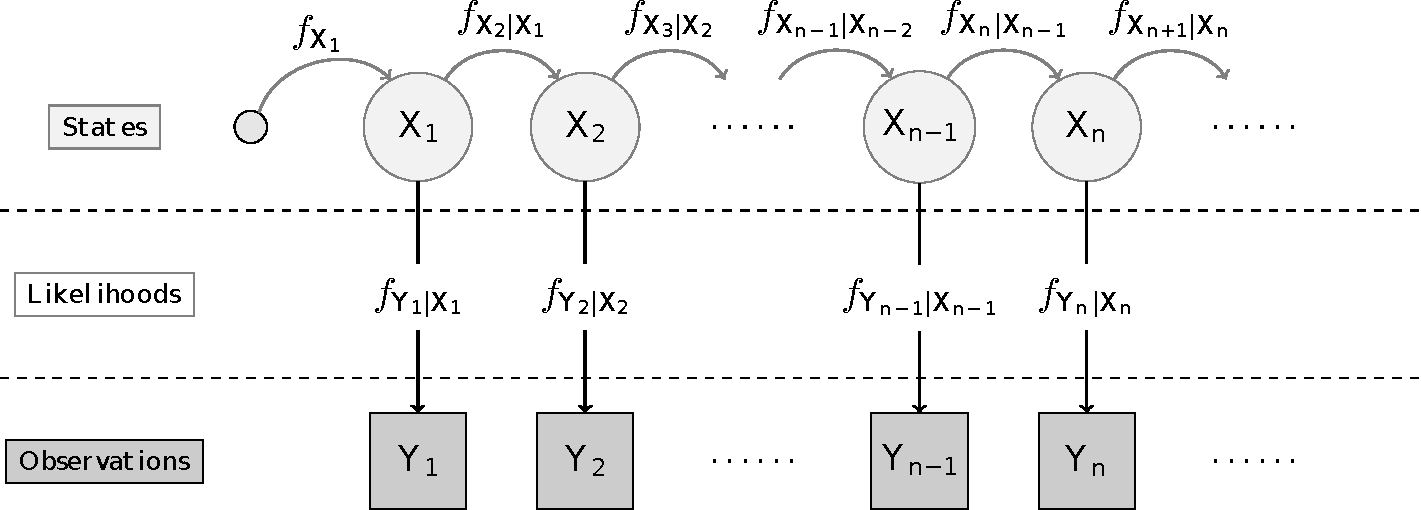
\includegraphics[width=\textwidth]{hidden_markov}

	Conditional pdf $f_{\VX_n|\VY_n}$ \qquad Likelihood pdf $f_{\Y_n|\X_n}$\\
	State-transision pdf $f_{\X_n|\X_{n-1}}$\\
	\textbf{Estimation:}
	\begin{equation*}
		f_{\VX_n|\VY_n} \propto f_{\VY_n|\VX_n} \cdot \int_{\mathbb X} f_{\VX_n|\VX_{n-1}} \cdot f_{\VX_{n-1}|\VY_{n-1}} \diff \vec x_{n-1}
	\end{equation*}
\end{sectionbox}